\documentclass[a4paper,10pt]{article}

%linguagem
\usepackage[brazil]{babel}
%encodificação
\usepackage[utf8]{inputenc}
%biblioteca de matemática
\usepackage{amssymb,amsmath}
%pacote para codigo fonte
\usepackage{listings}
%figuras
\usepackage{graphicx}
%cores
\usepackage{color}
%paragrafo no inicio da secao
\usepackage{indentfirst}
%url
\usepackage{framed, url}
\usepackage{fancyvrb}

\usepackage{longtable}

\usepackage[table]{xcolor}
\newcommand{\p}{\cellcolor{blue}}
\usepackage{slashbox} % Linha diagonal na tabela

%define a cor "claro"
\definecolor{claro}{gray}{0.96}

%configurações do fancy verbatim
\fvset{frame=single, xleftmargin=-80pt, xrightmargin=-80pt}
%configurações do listings
\lstset{language=C,frame=trBL, numbers=left, xleftmargin=0pt, xrightmargin=0pt,breaklines=true, backgroundcolor=\color{claro}}

\begin{document}

\begin{titlepage}
\begin{center}


\includegraphics[scale=0.2]{imagens/UFMG.png}\\
\textsc{\LARGE Universidade Federal de Minas Gerais\\
	Departamento de Ciência da Computação}\\[1.5cm]

\textsc{\Large Redes de Computadores\\
	Trabalho Prático 3}\\[0.5cm]

\hrulefill \\[0.4cm]
{ \LARGE \bfseries sistema de mensagens}\\[0.4cm]

\hrulefill \\[1.5cm]
\vspace{7cm}
\begin{minipage}{0.4\textwidth}
\begin{flushleft} \large
\emph{Aluno:}\\
Pedro Araujo Pires \\
\end{flushleft}
\end{minipage}
\begin{minipage}{0.4\textwidth}
\begin{flushright} \large
\emph{Professor:}\\
Luis Felipe Menezes Vieira\\
\end{flushright}
\end{minipage}

\vfill

{\large \today}

\end{center}
\end{titlepage}


\tableofcontents
\pagebreak

\section{Introdução}

Já fazem muitos anos que não conseguimos pensar em um computador como uma
máquina isolada do mundo. As redes permitem a comunicação entre computadores, e
por consequência entre usuários. A Internet não nos deixa dúvidas.

\subsection{Modelo cliente-servidor}
Grande parte da comunicação entre processos é feita utilizando o modelo
cliente-servidor. Este modelo se baseia na ideia de que um processo (o cliente)
se conecta a outro (o servidor) para pedir ou enviar informações. Uma boa
analogia seria uma pessoa fazendo uma ligação telefônica para outra. A pessoa
que faz a ligação precisa de saber o número do telefone da outra, mas quem
recebe não sabe quem está ligando. Uma vez que a chamada é completada, ambas as
pessoas podem falar e/ou escutar. A figura \ref{fig:clienteservidor} ilustra
este modelo.

\begin{figure}[ht!]
\begin{center}
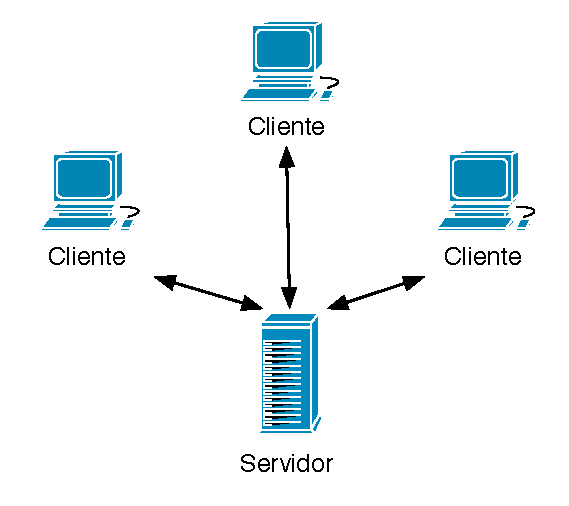
\includegraphics[scale=0.7]{imagens/clienteservidor.pdf}
\label{fig:clienteservidor}
\caption{Modelo cliente-servidor}
\end{center}
\end{figure}

\subsection{Protocolo TCP}
Para trocar informações entre computadores, além de estarem conectados, eles
precisam entender o que representam os dados enviados através da rede. Este é o
papel dos protocolos de rede. A Internet foi projetada através de camadas de
protocolos. Deste modo os desenvolvedores teriam liberdade para criar e mudar as
formas de comunicação sem precisar remodelar toda a estrutura da Internet. O
protocolo TCP - Transmission Control Protocol - fica na camada de transporte, como visto na figura
\ref{fig:protocolos}. Isto significa que ele é responsável por passar uma
mensagem vinda da rede para uma aplicação um nível acima. O TCP utiliza a forma
de fluxo de bytes para enviar mensagens e garante a confiabilidade do canal.
Desta forma a aplicação não precisa de se responsabilizar pelo tratamento de possíveis erros na
transmissão de pacotes entre o cliente e o servidor.

\begin{figure}[ht!]
\begin{center}
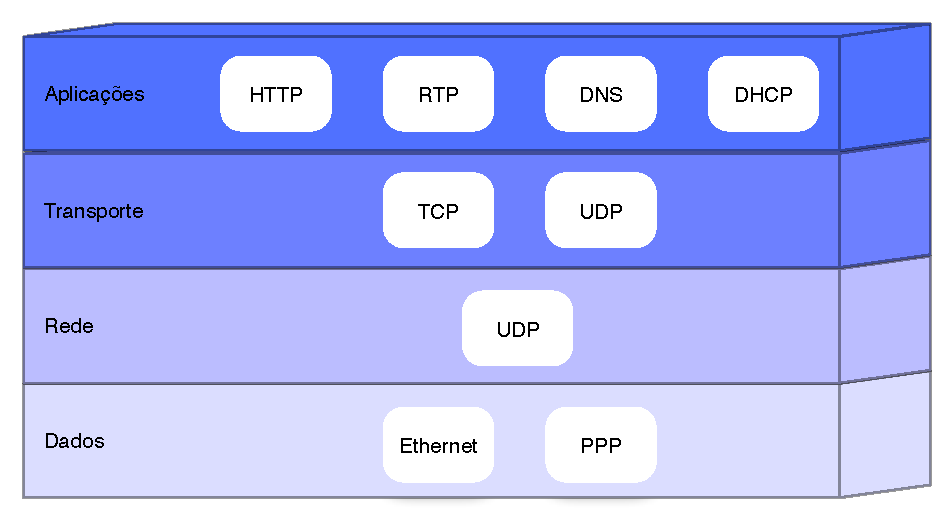
\includegraphics[scale=0.7]{imagens/protocolos.pdf}
\label{fig:protocolos}
\caption{Camadas de protocolos}
\end{center}
\end{figure}

\subsection{Sistema de mensagens}
O objetivo deste trabalho prático foi implementar um sistema de troca de mensagens
utilizando o modelo cliente-servidor e protocolo TCP. Para isso 3 aplicações
foram desenvolvidas:

\begin{itemize}
\item Servidor: Responsável por receber as conexões dos clientes, e fazer a
troca de mensagens entre os clientes.
\item Cliente de exibição: Exibe as mensagens destinadas a este cliente.
\item Cliente de envio: Envia mensagens para outros clientes.
\end{itemize}
\section{Implementação}

As mensagens enviadas pela aplicação são enviadas na forma de sequência de
bytes. Os 4 primeiros bytes são usados no cabeçalho. Os bytes subsequentes contêm o corpo da
mensagem, que pode ter até 140 caracteres. O formato do cabeçalho é descrito a
seguir:

\begin{itemize}
 \item \textbf{Tipo:}
  \begin{itemize}
    \item OI: Mensagem utilizada para um cliente se identificar para o
    servidor, e abrir uma conexão entre os dois.
    \item TCHAU: Mensagem especial para o cliente dizer ao servidor que
    vai fechar a conexão.
    \item MSG: Mensagem contendo um texto que pode ser enviado para um
    cliente específico ou para todos os clientes conectados ao servidor.
  \end{itemize}
 \item \textbf{Origem:} ID do cliente que enviou a mensagem.
 \item \textbf{Destino:} ID do cliente de destino.
 \item \textbf{Tamanho:} Tamanho do corpo da mensagem.
\end{itemize}

\begin{figure}[ht!]
\begin{center}
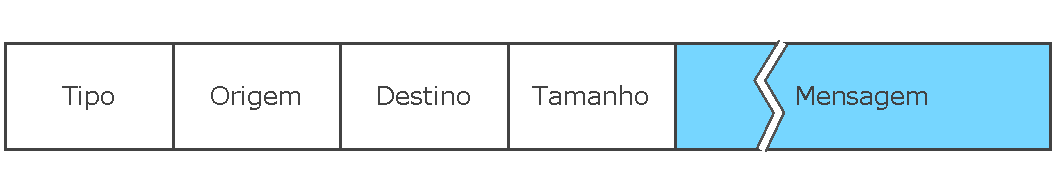
\includegraphics[scale=0.6]{imagens/mensagem.pdf}
\label{fig:mensagem}
\caption{Formato da mensagem}
\end{center}
\end{figure}

\section{Conclusões}

O trabalho foi de grande importância para conhecer a complexidade na
implementação de servidores que suportam conexões de vários clientes
simultaneamente. Também foi possível estudar e implementar o temporizador
utilizando sinais e funções de manipulação de tempo da biblioteca padrão do
Unix. A teoria envolvida neste trabalho é bem simples, entretanto a implementação possui vários detalhes de funcionamento que a
torna complexa de se codificar.

\clearpage
\begin{thebibliography}{99}
\bibitem{howto} \url{http://www.linuxhowtos.org/C_C++/socket.htm}
\bibitem{slide} \url{http://www.slideshare.net/jignesh/socket-programming-tutorial}
\bibitem{chat} \url{http://beej.us/guide/bgnet/output/html/multipage/clientserver.html}
\end{thebibliography}

\end{document}
